\documentclass[a4paper]{article}
\usepackage{iwslt15,amssymb,amsmath,epsfig}
\usepackage{siunitx, diagbox}
\setcounter{page}{1}
\sloppy		% better line breaks
%\ninept
%SM below a registered trademark definition
\def\reg{{\rm\ooalign{\hfil
     \raise.07ex\hbox{\scriptsize R}\hfil\crcr\mathhexbox20D}}}

%% \newcommand{\reg}{\textsuperscript{\textcircled{\textsc r}}}

\title{Digit String Recognition}

%%%%%%%%%%%%%%%%%%%%%%%%%%%%%%%%%%%%%%%%%%%%%%%%%%%%%%%%%%%%%%%%%%%%%%%%%%
%% Please make sure to keep technical paper submissions anonymous  !
%%%%%%%%%%%%%%%%%%%%%%%%%%%%%%%%%%%%%%%%%%%%%%%%%%%%%%%%%%%%%%%%%%%%%%%%%%
%\name{Firstname Lastname}
%%%%%%%%%%%%%%%%%%%%%%%%%%%%%%%%%%%%%%%%%%%%%%%%%%%%%%%%%%%%%%%%%%%%%%%%%%
%% If multiple authors, uncomment and edit the lines shown below.       %%
%% Note that each line must be emphasized {\em } by itself.             %%
%% (by Stephen Martucci, author of spconf.sty).                         %%
%%%%%%%%%%%%%%%%%%%%%%%%%%%%%%%%%%%%%%%%%%%%%%%%%%%%%%%%%%%%%%%%%%%%%%%%%%
\makeatletter
\def\name#1{\gdef\@name{#1\\}}
\makeatother
\name{{\em Lucas Steinmann, Leandro Piekarski, Hesham Hendy,}\\
      {\em Manuel Olk}}
%%%%%%%%%%%%%%% End of required multiple authors changes %%%%%%%%%%%%%%%%%

\address{Praktikum Neuronale Netze  \\Karlsruhe Institute of Technology, Germany \\
%{\small \tt firstname.lastname@iwslt.org}
}
%
\begin{document}
\maketitle
%
\begin{abstract}
This is a layout specification and template
definition for the paper of the IWSLT 2015 Conference. 
The format is essentially the one used for the IEEE ICASSP conferences.
\end{abstract}


%
\section{Introduction}
This template can be found on the conference 
website: \texttt{http://iwslt.org/}.
Please use either a MS-Word\reg\ or a \LaTeX\ format file
when preparing your submission. 

\section{Connectionist Temporal Classification}\label{sec:ctc}

The Loss has been calculated using CTC. It can be considered as an output layer of Neural network to deal with the following main problems:
\begin{itemize}
%\itemsep -1.3mm
\item The consumed time during the annotation process of the whole data set on digit level, which would be one to one correspondence between outputs and labels.
\item The limitation on the available information about the digits and its constraints which could be affected during the processing through many factors like noise or image resolution.
\end{itemize}
So These issues can be avoided through a function which is provided with the output matrix of the NN and the corresponding ground-truth (GT) text by trying all possible digit alignments between inputs and labels in the image and outputs at the end a classification at each input value by taking the highest score which conclude the real value. CTC uses the network to label the entire input sequence at once. This means the network can be trained with an unsegmented data set, and the final label sequence can be seen directly from the network output. The input of CTC is a sequence $y=y_{1},....y_{T}$ from a recurrent neural network with m inputs and n outouts, where T is the sequence length, For instance for an input squence y of length T, definde a RNN with m inputs, n ouputs and weight vektor w as a continous map $N_w$: ($\mathbb{R^m}$) $\rightarrow$  ($\mathbb{R^n}$).Then the first step called Encoding can be initiated through inserting randomly a pseudo character called Blank denoted with {-} which must be inserted in case of digits duplication. For a given $y_{T}$ it gives us an output distribution over all possibilities.Then a conditional probability is defined as the sum of probabilities of all $\pi$ which are mapped by F onto I:
\begin{equation}
p( I | y)=\sum_{\pi \in F(I)} p( \pi | y )
\label{eq3}
\end{equation}
where the conditional probability of $\pi$ is defined as: 
\begin{equation}
p( \pi | y ) =\prod_t^T y_{\pi_{t}}
\label{eq3}
\end{equation}
The probability $p( \pi | y )$ of a particular path or respectively label observing is the product of all the softmax outputs "digit scores" $y_{\pi_{t}}$ over time T for one alignment. The function takes the negative log probability of ground truth all the training examples in training set D
\begin{equation}
\sum_{(i,y)_{\in D}} - \log  p( I | Y )
\label{eq3}
\end{equation}
where y is the sequence produced by the recurrent layers from x. Then we should update the network through back propagation. By decoding, the function calculates the best path by taking the most likely character per time-step and undoes the encoding measures by first removing duplicate characters and then removing all blanks from the path and as a result remains the recognized text \cite{CTC}.


\section{Recurrent Neural Network}\label{sec:rnn}
Based on the human fact that we do not need to rethink from scratch rather building up on the available results, Recurrent Neural Network has been developed to solve this issue with the normal neural network using connected chunks of neural network. The information can be passed over the chunks in a loop intimately, but It shouldn’t go so far back to avoid gradient vanish problem during the parameter optimization especially by a small number of Iterations. So LSTM should be used instead of the RNN.The LSTM short of learning long-term dependencies does have the ability to remove or add information to the cell state, carefully regulated by 4 specified mechanism called gates:
\begin{itemize}
%\itemsep -1.3mm
\item Forgetting mechanism.
\item Saving (remembering) mechanism.
\item Learning mechanism.
\item Focusing long-term memory into working memory which is the next short memory.
\end{itemize}
LSTM transforms its memory in a very precise way using these mechanisms for which pieces of information to remember, which to update, and which to learn. This helps it keep track of information over longer periods of time. At the same time, the future events should be also considered, therefore the network will be handle that trainings in the opposite direction, i.e each training sequence forwards and backwards to two separate LSTM layer, und that has been called bidirectional LSTM. 

\section{Approach}\label{sec:approach}

\subsection{Architecture}\label{subsec:architecture}
This section covers the architecture, with which we achieved our best results, which are presented in \autoref{sec:evaluation}. Our architecture is based on a published architecture~\cite{CTC} which achieved the best performance in the competition ICFHR 2014~\cite{icfhr_competition}.

The task of digit string recognition poses several challenges across different machine learning disciplines.
On the one hand, the input image is a high-dimensional tensor (after resizing $120\times50\times3$).
As a consequence, the input will have a low information density and considerable amount of noise.
A proven neural network architecture class for processing images are convolutional neural networks (CNN).
More specifically, we employ a smaller variant of the Residual Network (ResNet)~\cite{ResNet} architecture.
See \autoref{fig:resblock} for a detailed view of our implementation of the residual architecture.
After every convolutional layer we performed batch normalization~\cite{batchnorm} to prevent internal covariance shift and accelerate training.
This first step in our architecture can be seen as an \emph{encoder}, mapping the input image to a 3 dimensional tensor with lower spatial dimensions ($15 \times 6$) but more channels (512).

We then interpret the output as a sequence along the horizontal axis.
For simplicity we have designed the horizontal output dimension of the encoder to be equal to the maximal sequence length.
In this case every column matrix (of size $6 \times 512$ represents one sequence element).
If this is not possible or the sequence length should be variable without changing the encoder, a linear projection can be used to increase or decrease the horizontal dimension.

The remaining task is to decode this tensor by labeling every element of the sequence with a digit or blank.
We output scores for every digit and blank for each element in the sequence.
The output dimensionality of every label is therefore 11.
The class network architecture we use for this task are called recurrent neural networks (RNNs).
As described in \autoref{sec:rnn}, vanilla RNNs suffer from the vanishing gradient problem.
We therefore use long short term memory (LSTM)~\cite{LSTM}, which mitigate this issue.
LSTMs can be stacked by using the output of the previous layer as input to the next layer.
We use two layer LSTMs to allow the network to learn a more complex function.
In addition we use bidirectional LSTMs (BiLSTM), which are independently applied to the original sequence and the reversed sequence and combine their outputs by addition.
Our BiLSTM outputs a 100-d vector at every time step.
Finally a linear layer is used to reduce this dimension to 11.
During training we use log-softmax to prepare the output for calculation of the CTC-Loss.
When inferring labels we select the element with the highest output using the argmax operator at each time step.
The full architecture is shown in \autoref{fig:architecture}.

\begin{figure}
    \begin{center}
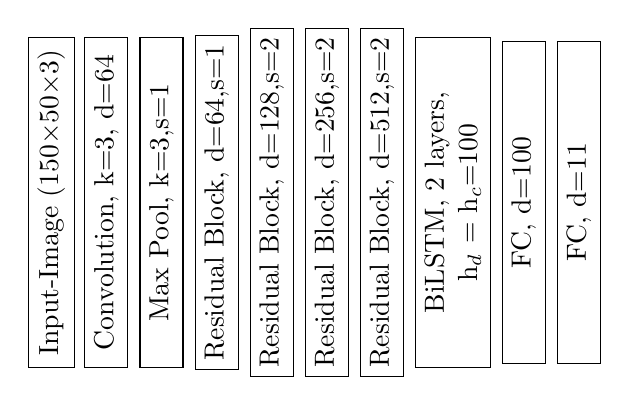
\begin{tikzpicture}
    \node[rectangle,minimum width=4.2cm,draw,rotate=90] at (0,2.1) (input) {Input-Image (150$\times$50$\times$3)};
    \node[rectangle,minimum width=4.2cm,draw,rotate=90] at (0.7,2.1) (conv1) {Convolution, k=3, d=64};
    \node[rectangle,minimum width=4.2cm,draw,rotate=90] at (1.4,2.1) (pool1) {Max Pool, k=3,s=1};
    \node[rectangle,minimum width=4.2cm,draw,rotate=90] at (2.1,2.1) (res1) {Residual Block, d=64,s=1};
    \node[rectangle,minimum width=4.2cm,draw,rotate=90] at (2.8,2.1) (res2) {Residual Block, d=128,s=2};
    \node[rectangle,minimum width=4.2cm,draw,rotate=90] at (3.5,2.1) (res3) {Residual Block, d=256,s=2};
    \node[rectangle,minimum width=4.2cm,draw,rotate=90] at (4.2,2.1) (res4) {Residual Block, d=512,s=2};
    %\node[rectangle,minimum width=2.1cm,draw,rotate=90] at (5.25,1.05) (reverse) {reverse};
    \node[rectangle,minimum width=4.2cm,draw,rotate=90,align=center] at (5.1,2.1) (bilstm) {BiLSTM, 2 layers, \\ $\text{h}_d$ = $\text{h}_c$=100};
    \node[rectangle,minimum width=4.1cm,draw,rotate=90] at (6,2.1) (fc1) {FC, d=100};
    \node[rectangle,minimum width=4.1cm,draw,rotate=90] at (6.7,2.1) (fc2) {FC, d=11};
\end{tikzpicture}
\caption{Schematic of our architecture. Dropouts and batch normalizations are omitted for brevity.}\label{fig:architecture}
\end{center}
\end{figure}
\begin{figure}
    \begin{center}
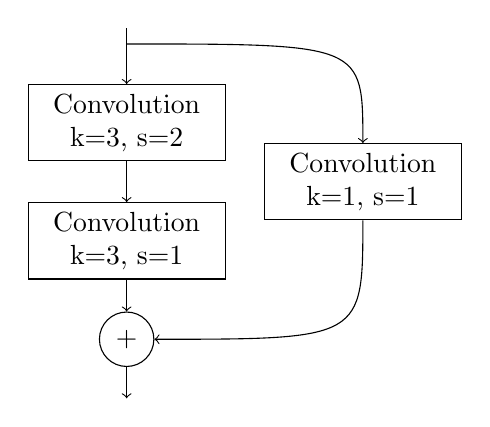
\begin{tikzpicture}
    \node[rectangle, minimum width=2.5cm,draw,align=center] at (0,-1) (conv1) {Convolution\\ k=3, s=2};
    \node[rectangle, minimum width=2.5cm,draw,align=center] at (0,-2.5) (conv2) {Convolution\\ k=3, s=1};
    \node[rectangle, minimum width=2.5cm,draw,align=center] at (3,-1.75) (resconv) {Convolution\\ k=1, s=1};
    \node[circle,draw,align=center] at (0,-3.75) (add) {$+$};
    \draw[->] (0,0.2) -- (conv1);
    \draw[->] (conv1) -- (conv2);
    \draw[->] (0,0) .. controls (3,0) .. (resconv);
    \draw[->] (conv2) -- (add);
    \draw[->] (resconv) .. controls (3,-3.75) .. (add);
    \draw[->] (add) -- (0,-4.5);
\end{tikzpicture}
\caption{Schematics of a residual block in our architecture. If the output dimension does not change (as in our first residual block, the linear mapping in the residual path is not required and therefore omitted. Furthermore does the first residual block use a stride of 1 instead of 2.}\label{fig:resblock}
\end{center}
\end{figure}
\subsection{Training}\label{subsec:training}

We divided our training in epochs.
In each epoch we observe every training sample once.
Each sample is randomly manipulated by different data augmentation methods as described in \autoref{Datasets}.
We normalized each sample by channel-wise whitening (subtracting dataset mean color value and dividing by dataset variance).
The Adam~\cite{Adam} is used to minimize the CTC loss per batch.
We found a batch-size of 32 to deliver the best results.
Higher batch-sizes resulted into very slow learning, due to seldom updates, while lower batch-sizes did had less parallelization on GPU and where therefore slower to compute.
Increasing the step size when using higher batch-sizes did not speed up training either.
We suspect that the loss function surface is shaped in a way, such that higher variance gradient descent (as achieved by lower batch-sizes) results in faster convergence.

For hyper-parameter optimization we split our training data in a training and validation dataset, whereby 80\% of the training data is used for training and the rest is only used to evaluate the model performance.


\section{Evaluation}\label{sec:evaluation}

\subsection{Metrics}

To evaluate the performance of the models two metrics are utilized. The first
one is the Levenshtein distance, also known as edit distance. The edit distance
as depicted by Fig.~\ref{fig_edit_distance} calculates how many changes among
insertions, deletions and substitutions are necessary to transform one string
into another \cite{rice_edit_dist}. In this work all changes are weighted the
same. The second metric is accuracy, which considers a prediction correct only
if all characters match the label characters in the correct position. Originally
\cite{icfhr_competition} considers from TOP-1 to TOP-3 submissions in case of
accuracy, however this work considers only the TOP-1 network output. For the
final results of the trained models in this section only accuracy is displayed
since it is a harder metric and the only one which can be compared with the
baseline results. 

\begin{figure}[t]
%\centerline{\epsfig{figure=figure,width=40mm}}
\centerline{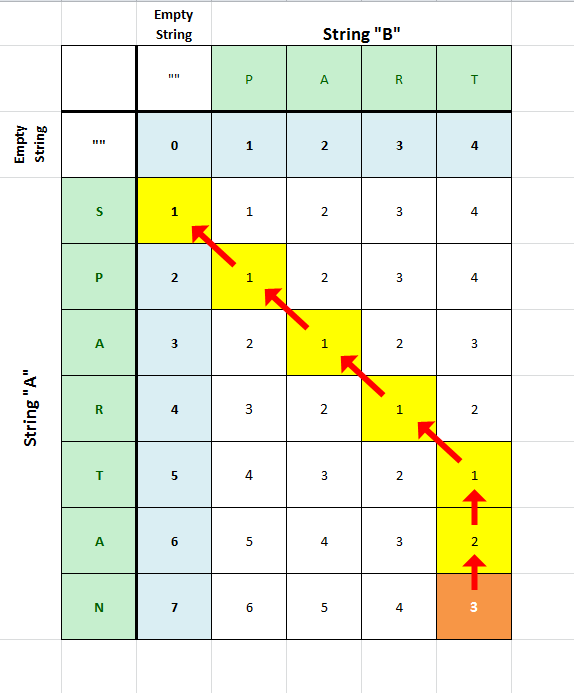
\includegraphics[width=40mm]{images/edit_distance}}
\caption{{\it Example of edit distance for words 'part' and 'spartan' \cite{rice_edit_dist}.}}  
\label{fig_edit_distance}
\end{figure}

\subsection{Model performance}

The implemented model is similar to the one proposed by Zhan et al.
\cite{zhan2017}, therefore its results are used as a reference of what can be
achieved with an architecture using CNN + RNN-CTC. For each of the provided
datasets, the model is trained for 100 epochs with Adam as optimizer, learning
rate of \num{1e-04} and batch size equal to 16. The provided sets are already
separated into training and test data, thus the training data was split further
into 80\% of it for training and 20\% for validation. Table
\ref{table_zhan_interpretation} summarizes the comparison between the baseline
and the used model. In each case of this comparison models were trained and
tested only with data of the referenced dataset. 

\begin{table}
\caption{\label{table_zhan_interpretation} {\it Overall comparison between implementations.}}
\vspace{2mm}
\centerline{
\begin{tabular}{*{4}{|c}|}
\hline
Methods & 
CAR-A &
CAR-B & 
CVL\\
\hline \hline 
Zhan el al. 2017 & 0.8975 & 0.9114 & 0.2707 \\
Our 'interpretation' & 0.9014 & 0.9084 & 0.2550 \\
\hline
\end{tabular}}
\end{table}

Given the fact that the model is able to perform well on CAR-A and CAR-B,
experiments with cross-validation with data from different sets are made to
evaluate if the reason for poor performance on CVL is the architecture or the
data. Table \ref{table_different_sets} contains the results for models which
were trained with datasets on the first line and tested against datasets on the
first column. Considering only CAR-A and CAR-B, the best results are obtained by
training and testing with data within a same set. The more interesting results
are for CVL tests, as it has the worst performance when using its own training
set and receives big performance improvements achieving almost 60\% if tested on
a model which was trained exclusively with CAR-B data.  

\begin{table}
\caption{\label{table_different_sets} {\it Performance on different sets.}}
\vspace{2mm}
\centerline{
\begin{tabular}{*{4}{|c}|}
\hline
\backslashbox{Tested}{Trained} & 
CAR-A &
CAR-B & 
CVL\\
\hline \hline 
CAR-A & \textbf{0.9014} & 0.7315 & 0.002 \\
CAR-B & 0.8434 & \textbf{0.9084} & 0.006 \\
CVL & 0.3019 & \textbf{0.5804} & 0.2550 \\
\hline
\end{tabular}}
\end{table}

A further idea to improve the CVL performance follows the principle 'more data
is always better'. As observed in the previous experiments as well as for
reasons discussed in the data analysis in Section \ref{introduction}, the CVL
test data is not represented well by its training data, especially regarding the
small amount of different string labels. The idea is therefore to adopt the
whole training data of CAR-A plus CAR-B to train the model from scratch and
additionally fine-tune it on CVL. Taken into account from the previous
experiments that the architecture is able to generalize well and to maximize the
amount of training data, no validation data is used in these experiments. Apart
from the lacking train-validation split, all the parameters remain the same. For
fine-tuning, all weights are trained for extra 20 epochs exclusively on CVL.
Table \ref{table_fine_tuning} contains the results for these experiments.

The model trained on CAR-A+CAR-B without CVL data surpasses both the
performances of models trained exclusively on these sets as well as the
previously best CVL performance. By fine-tuning the model on CVL however, the
CVL test performance achieved almost 76\%, which compared to the results in
\cite{icfhr_competition} means a second best CVL performance losing only to
BeiJing et al. \cite{icfhr_competition}. 

\begin{table}
\caption{\label{table_fine_tuning} {\it Performance using more than one set + fine-tuning.}}
\vspace{2mm}
\centerline{
\begin{tabular}{*{3}{|c}|}
\hline
\backslashbox{Tested}{Trained} & 
CAR-A + CAR-B &
CVL (fine-tuning)\\
\hline \hline 
CAR-A & \textbf{0.9127} & 0.0565 \\
CAR-B & \textbf{0.9408} & 0.4733 \\
CVL & 0.5913 & \textbf{0.7579} \\
\hline
\end{tabular}}
\end{table}

\subsection{Performance impact of the RNN}

For the purpose of checking what is the impact of the LSTM for sequence labeling
in this model, experiments are made by removing the bidirectional LSTM. For a
reasonable comparison, the model is almost identical to the one depicted by
Fig.~\ref{fig:architecture}, however without the BiLSTM block. 

\begin{table}
\caption{\label{table_different_sets_no_rnn} {\it Performance on different sets without LSTM.}}
\vspace{2mm}
\centerline{
\begin{tabular}{*{4}{|c}|}
\hline
\backslashbox{Tested}{Trained} & 
CAR-A &
CAR-B & 
CVL\\
\hline \hline 
CAR-A & \textbf{0.8884} & 0.7185 & 0.002 \\
CAR-B & 0.7926 & \textbf{0.8882} & 0.026 \\
CVL & 0.3392 & 0.4561 & \textbf{0.5676} \\
\hline
\end{tabular}}
\end{table}

As seen in Table \ref{table_different_sets_no_rnn}, the results on datasets
CAR-A and CAR-B are slightly worse, suggesting that these datasets do have small
digit contexts which can benefit from an LSTM. More interestingly, the results
when using only the CVL dataset can be significantly improved and is on par with
other more successful approaches at the ICHFR2014 competition
\cite{icfhr_competition}. This suggests the LSTM is overfitting with the small
string variance provided by the CVL dataset and has therefore a big negative
impact. 

\subsection{Error cases}

In order to have a better understanding of the mistakes the network makes, some
of the errors during test are collected. Most of the errors fall into four
classes. The first class is represented by Fig.~\ref{fig_error1}, in which the
left border is misclassified as the digit '1', resulting in a prediction '175'
versus label '75'. Right borders can also be misclassified. A second class is as
depicted by Fig.~\ref{fig_error2}, in which the digits cannot be easily
classified correctly even by humans. In this case the network predicts '400' for
a label '500'. The third class of identified errors is illustrated by
Fig.~\ref{fig_error3}. Due to the fact that the pictures do not include
exclusively digits, symbols such as commas can be confused with the digit '1',
despite the training to classify all strange symbols as 'blank'. The last error
class is pictured by Fig.~\ref{fig_error4}. Given the CNN output, the input
picture is divided in 15 parts to be classified by the RNN. A problem also
occurs thereby if irrelevant symbols occupy too much space in a way that a
single digit is too small inside one of these parts. For the example the
prediction was '381', which suggests that the digits '29' are merged during the
feature extraction. 

\begin{figure}[t]
    \centering
  \subfloat[Border\label{fig_error1}]{%
       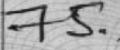
\includegraphics[width=0.2\linewidth]{images/error1}}
    \hfill
  \subfloat[Bad digits\label{fig_error2}]{%
        
\includegraphics[width=0.2\linewidth]{images/error2}}
    \hfill
  \subfloat[Symbols\label{fig_error3}]{%
        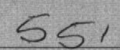
\includegraphics[width=0.2\linewidth]{images/error3}}
    \hfill
  \subfloat[Receptive field\label{fig_error4}]{%
        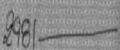
\includegraphics[width=0.2\linewidth]{images/error4}} \\
  \caption{{\it Examples of test errors}}
  \label{fig_methods} 
\end{figure}

Most of these errors can be probably avoided by investing more time into
preprocessing the images, which is neglected in this work in favor of an
end-to-end approach. Any extra preprocessing for such images requires feature
engineering to remove irrelevant symbols by for example, searching for contours
which are more likely to belong to digits as in Fig.~\ref{fig_preproc}. As a
consequence the deep learning model would require less effort and complexity.  

\begin{figure}[t]
%\centerline{\epsfig{figure=figure,width=40mm}}
\centerline{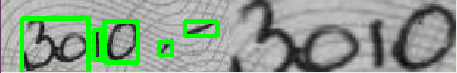
\includegraphics[width=40mm]{images/preproc}}
\caption{{\it Digit contour detection}.}  
\label{fig_preproc}
\end{figure}

\section{Lessons learned}

Of the many lessons learned during the development of this work, the most
important is to recognize when overfitting is happening. Divergences between
training and validation performance tend to happen but if they are too big a
thorough analysis of the possible causes is necessary. Data augmentation and
regularization methods do help but are not enough to overcome highly divergent
performances, which are more likely caused by a wrong approach. Models for more
complex tasks have so many parameters that is easy for them to memorize the
training set completely without any generalization capability given enough
epochs. 

A second lesson is to analyze carefully which type of information is passed to
the LSTM input gates. Just reshaping tensors output by the CNN to fit the LSTM
input shape without any reasonable criteria does not deliver any valuable
results. At first, it is not clear what to use as input in the presented problem
since the sequence aspect is not instantly recognized as in problems which have
for example image sequences as input or text sentences. Following the intuition
of splitting the classification along the image width dimension, the LSTM time
steps must also match this idea for learning effectively.

\section{Conclusions}\label{sec:conclusion}

This paper describes the implementation of a previously proposed full end-to-end
architecture based on CNN + RNN-CTC to solve the digit string recognition
problem. Cross-validation with different datasets is done to identify possible
improvements due to not representative data and delivers impressive results.
Finally, the RNN part is removed from the original model and shows that better
results can be achieved on datasets with small label variance in a task which
in theory does not have context dependence. 


\section{Acknowledgements}
The IWSLT 2015 organizing committee would like to thank the
organizing committees of INTERSPEECH 2004 for their
help and for kindly providing the template files.

%
\bibliographystyle{IEEEtran}

%\begin{thebibliography}{10}
\bibitem[1]{ES1} Smith, J. O. and Abel, J. S., 
``Bark and {ERB} Bilinear Transforms'', 
IEEE Trans. Speech and Audio Proc., 7(6):697--708, 1999.  
\bibitem[2]{ES2} Lee, K.-F., Automatic Speech Recognition: 
The Development of the 
SPHINX SYSTEM, Kluwer Academic Publishers, Boston, 1989.
\bibitem[3]{ES3} Rudnicky, A. I., Polifroni, Thayer, E. H.,
 and Brennan, R. A.  
"Interactive problem solving with speech", J. Acoust. Soc. Amer., 
Vol. 84, 1988, p S213(A).
\end{thebibliography}
\bibliography{bib_}

\end{document}

